\documentclass{article}
\usepackage{listings}
\usepackage{color}
\usepackage{keyval}
\definecolor{dkgreen}{rgb}{0,0.6,0}
\definecolor{gray}{rgb}{0.5,0.5,0.5}
\definecolor{mauve}{rgb}{0.58,0,0.82}
\usepackage{bookmark}
\usepackage{amsmath}
\usepackage{geometry}
\usepackage{hyperref}
\usepackage{listings}
\usepackage{xcolor}
\usepackage{graphicx}
\usepackage{amsfonts}

\lstset{
  basicstyle=\footnotesize, 
  numbers=left, 
  numberstyle=\tiny\color{gray}, 
  stepnumber=1,
  numbersep=5pt, 
  backgroundcolor=\color{white},
  showspaces=false,
  showstringspaces=false,
  showtabs=false,
  frame=shadowbox,
  rulecolor=\color{black},
  tabsize=2,
  captionpos=b,
  breaklines=true, 
  breakatwhitespace=false, 
  title=\lstname,
  keywordstyle=\color{blue},
  commentstyle=\color{dkgreen},
  escapeinside={\%*}{*)}, 
  morekeywords={*,...} 
}

\begin{document}

The algorithm is test in cases where the size of $S$ ranges from 0 to 100, and in the set the elements are just $1,2,3,....len(S)$. Because in this problem $n$ is also a factor that will influence the time, in every case $n$ is set to be $\lfloor \frac{sum(S)}{2} \rfloor$

And the result is shown in the graph below:

\begin{figure}[h]
    \centering
    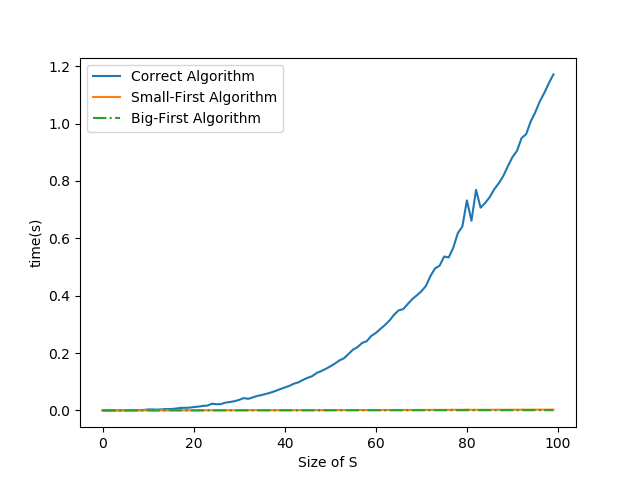
\includegraphics[scale=0.5]{1.png}
\end{figure}

It is the time to perform 50 same algorithm repeatedly. It can be seen that the proper algorithm is much more time-costing than the two other algorithms. It is obvious since the correct algorithm has a $O(len(s)\times n)$ time complexity where the other two only need $O(nlogn)$. 

Because in some cases the big-first and small-first algorithm could also give us correct or nearly correct solutions, we can sometime use these two when time efficiency is highly needed.
\end{document}